\begin{figure}
  \centering
  \begin{subfigure}[b]{0.5\textwidth}
    \begin{tikzpicture}
      \node[inner sep=0pt] (img1) at (0.0\textwidth, -0.0\textwidth)
           {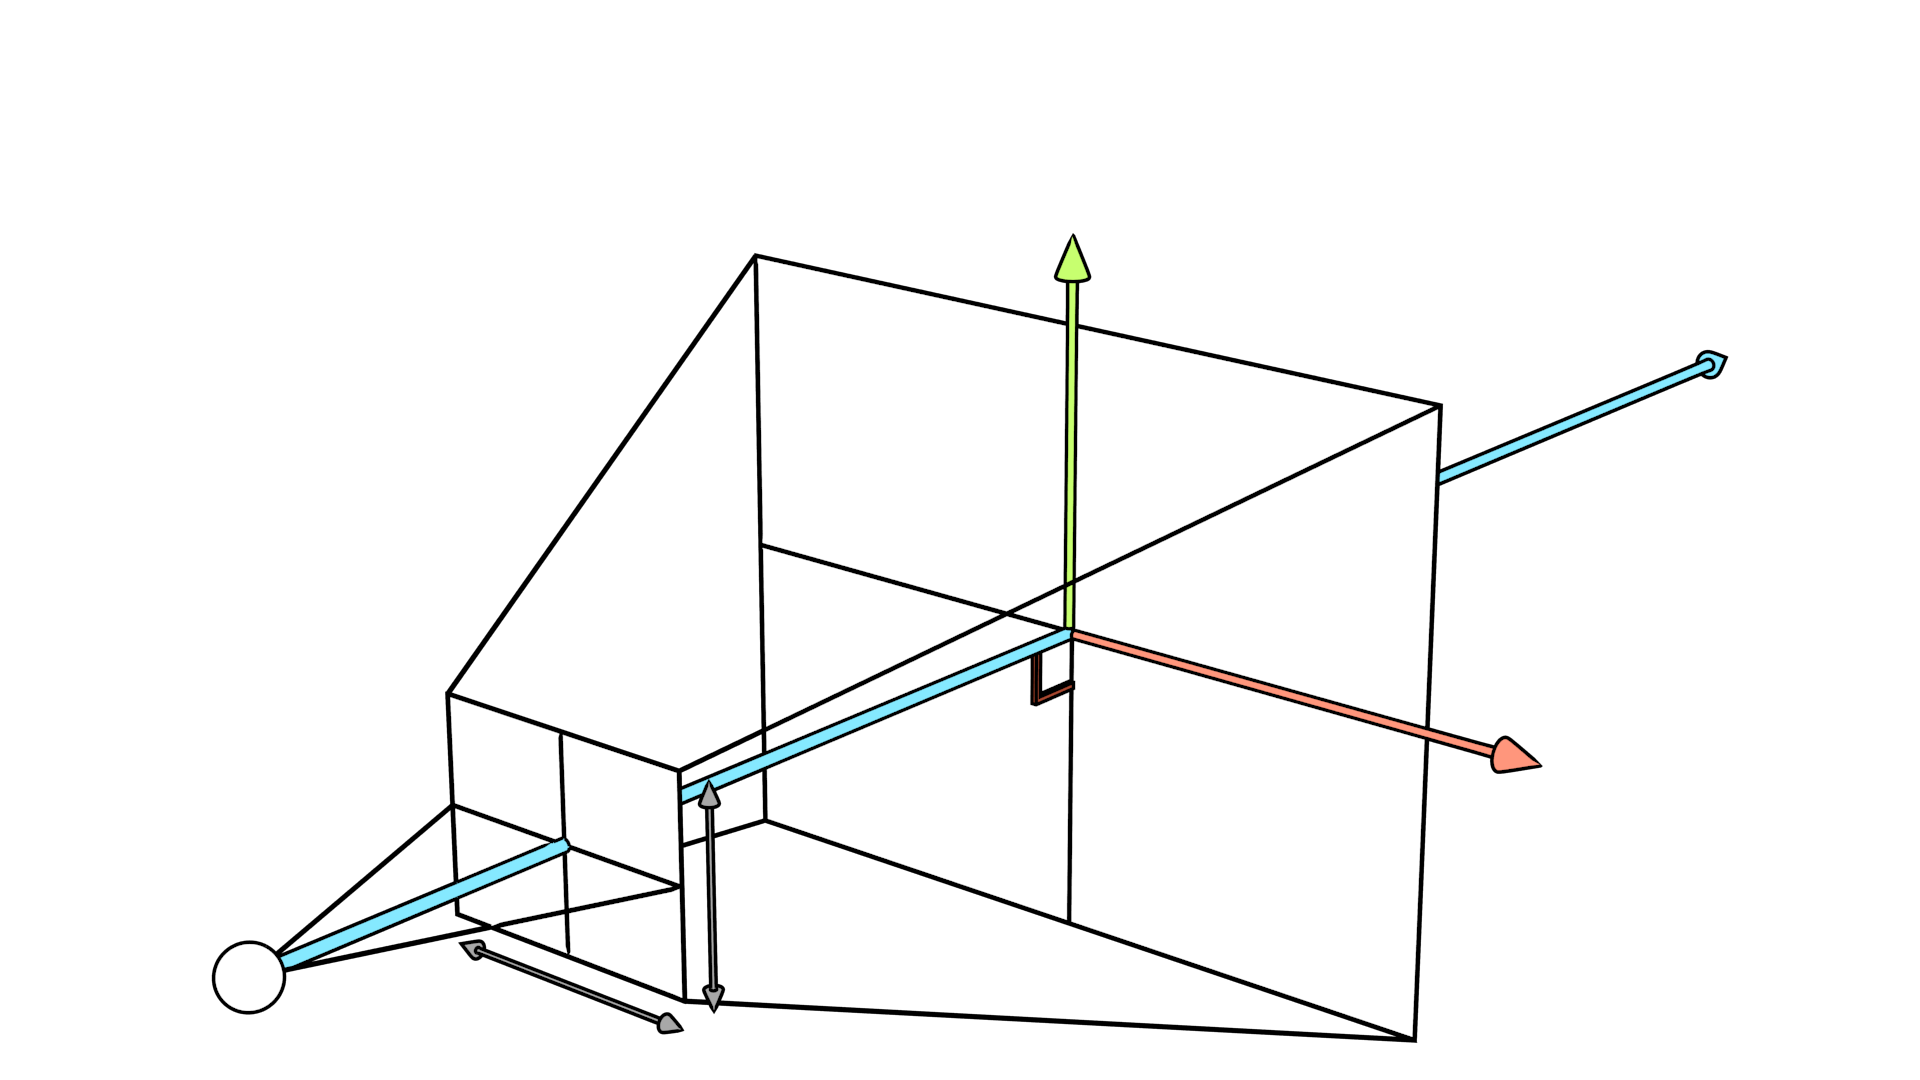
\includegraphics[width=\textwidth]{./img/raw/camera/camera_1.png}};

      \node[] (camera-origin) at (-0.35\textwidth, -0.28\textwidth) {$\mathcal{O}_\mathtt{camera}$};
      \node[] (camera-origin) at (-0.32\textwidth, -0.14\textwidth) {$\theta$};
      \node[] (camera-origin) at (-0.24\textwidth, -0.25\textwidth) {$\mathit{w}$};
      \node[] (camera-origin) at (-0.1\textwidth, -0.18\textwidth) {$\mathit{h}$};
      \node[] (camera-origin) at (0.056\textwidth, .19\textwidth) {up};
      \node[] (camera-origin) at (0.39\textwidth, .12\textwidth) {kijkrichting};
      \node[] (camera-origin) at (-0.335\textwidth, .08\textwidth) {zichtfrustum};
      \node[] (camera-origin) at (-0.36\textwidth, -.08\textwidth) {z-near};
      \node[] (camera-origin) at (-0.21\textwidth, .15\textwidth) {z-far};
    \end{tikzpicture}
    \caption{Met kijkrichting vector.}
    \label{fig:cm-camera:vec}
  \end{subfigure}%
  \begin{subfigure}[b]{0.5\textwidth}
    \begin{tikzpicture}
      \node[inner sep=0pt] (img1) at (0.0\textwidth, -0.0\textwidth)
           {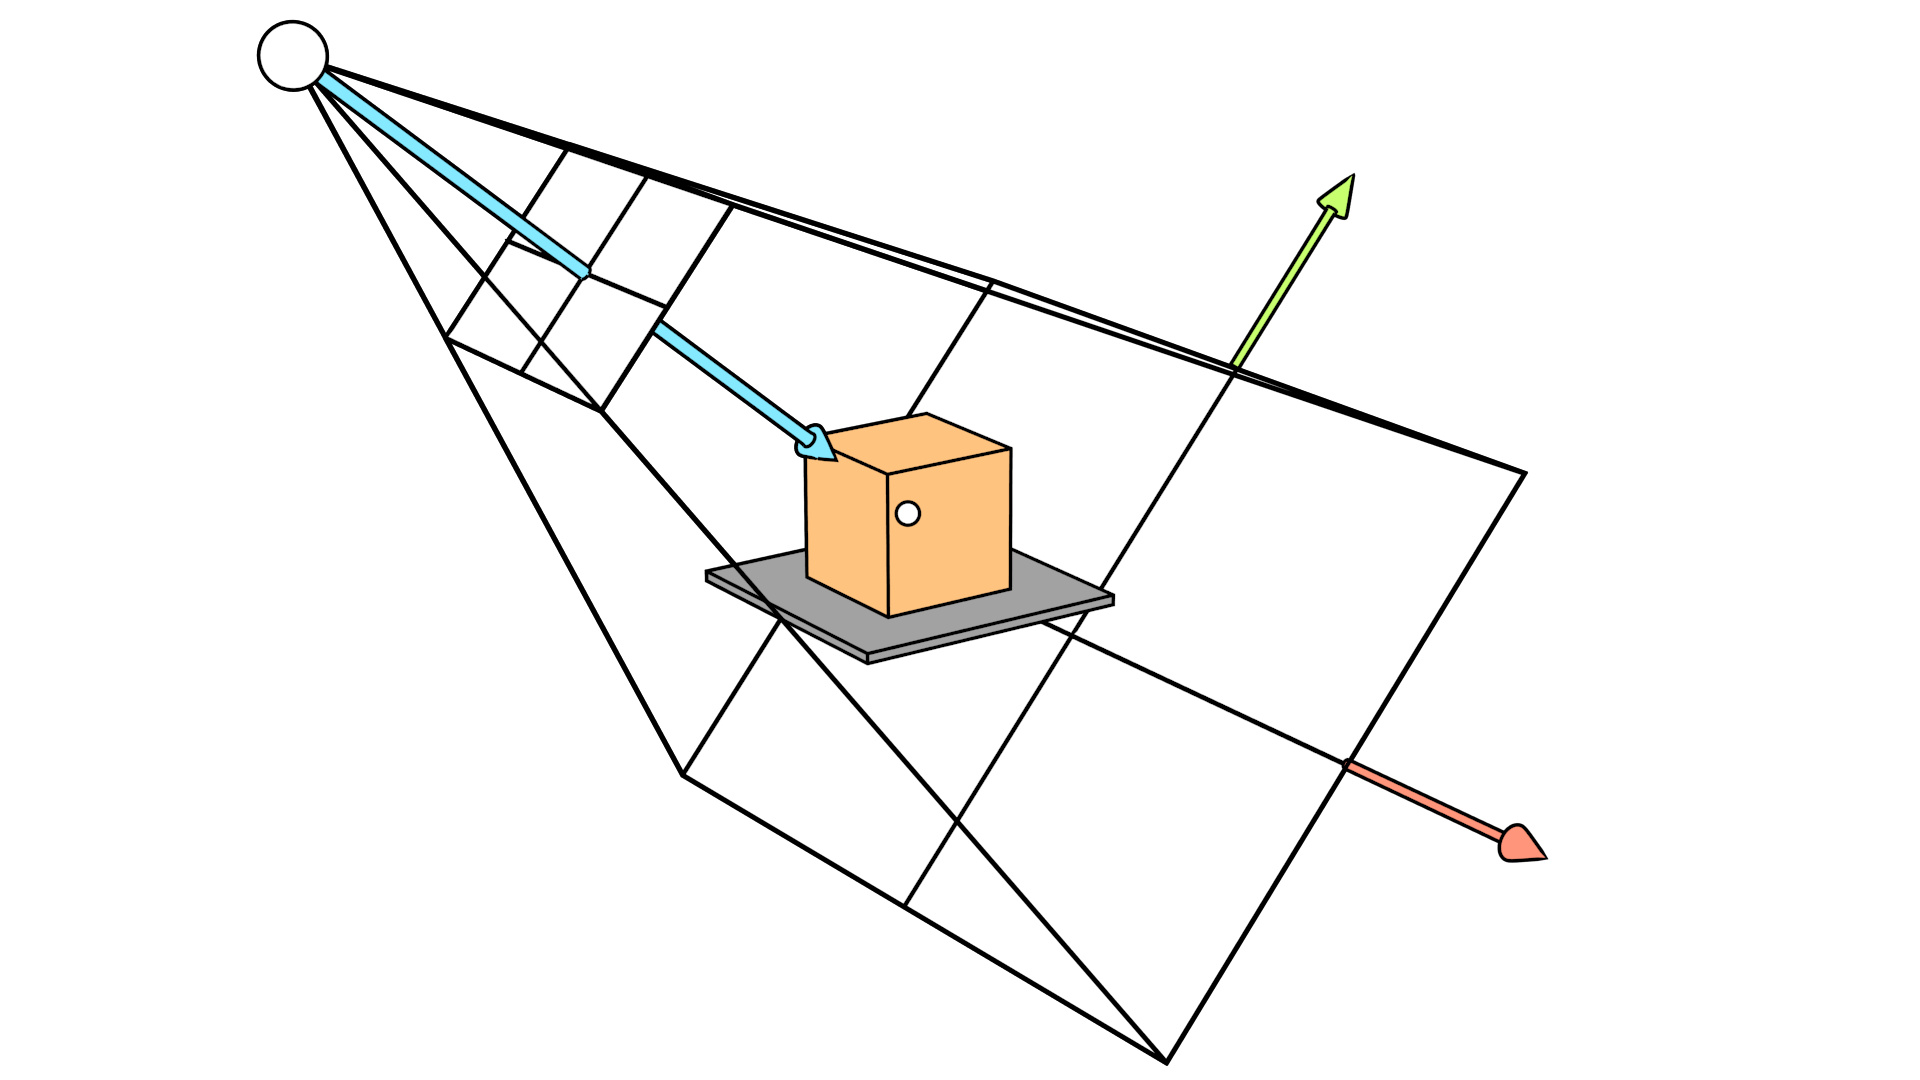
\includegraphics[width=\textwidth]{./img/raw/camera/camera_2.png}};

      \node[] (camera-origin) at (-0.35\textwidth, 0.305\textwidth) {$\mathcal{O}_\mathtt{camera}$};
      \node[] (camera-origin) at (0.05\textwidth, .08\textwidth) {center};
      \node[] (camera-origin) at (0.2\textwidth, .225\textwidth) {up};
    \end{tikzpicture}
    \caption{Met center-punt.}
    \label{fig:cm-camera:vec}
  \end{subfigure}
  \caption{Het Cameramodel.}
  \label{fig:cm-camera}
\end{figure}
